%%% Template originaly created by Karol Kozioł (mail@karol-koziol.net) and modified for ShareLaTeX use

\documentclass[a4paper,11pt]{article}

\usepackage[T1]{fontenc}
\usepackage[utf8]{inputenc}
\usepackage{graphicx}
\usepackage{xcolor}

\renewcommand\familydefault{\sfdefault}
\usepackage{tgheros}
\usepackage[defaultmono]{droidmono}

\usepackage{amsmath,amssymb,amsthm,textcomp}
\usepackage{enumerate}
\usepackage{multicol}
\usepackage{tikz}
% subfigures
\usepackage{caption}
\usepackage{subcaption}
\usepackage[toc,page]{appendix}


\usepackage{geometry}
\geometry{total={210mm,297mm},
left=25mm,right=25mm,%
bindingoffset=0mm, top=20mm,bottom=20mm}

\usepackage[
backend=biber,
style=alphabetic,
sorting=ynt
]{biblatex}

\addbibresource{bibliography.bib} % imports bibliography file


\linespread{1.3}

\newcommand{\linia}{\rule{\linewidth}{0.5pt}}

% custom theorems if needed
\newtheoremstyle{mytheor}
    {1ex}{1ex}{\normalfont}{0pt}{\scshape}{.}{1ex}
    {{\thmname{#1 }}{\thmnumber{#2}}{\thmnote{ (#3)}}}

\theoremstyle{mytheor}
\newtheorem{defi}{Definition}

% my own titles
\makeatletter
\renewcommand{\maketitle}{
\begin{center}
\vspace{2ex}
{\huge \textsc{\@title}}
\vspace{1ex}
\\
\linia\\
\@author \hfill \@date
\vspace{4ex}
\end{center}
}
\makeatother
%%%

% custom footers and headers
\usepackage{fancyhdr}
\pagestyle{fancy}
\lhead{}
\chead{}
\rhead{}
\lfoot{Assignment \textnumero{} 1}
\cfoot{}
\rfoot{Page \thepage}
\renewcommand{\headrulewidth}{0pt}
\renewcommand{\footrulewidth}{0pt}
%

% code listing settings
\usepackage{listings}
\lstset{
    language=Octave,
    basicstyle=\ttfamily\small,
    aboveskip={1.0\baselineskip},
    belowskip={1.0\baselineskip},
    columns=fixed,
    extendedchars=true,
    breaklines=true,
    tabsize=4,
    prebreak=\raisebox{0ex}[0ex][0ex]{\ensuremath{\hookleftarrow}},
    frame=lines,
    showtabs=false,
    showspaces=false,
    showstringspaces=false,
    keywordstyle=\color[rgb]{0.627,0.126,0.941},
    commentstyle=\color[rgb]{0.133,0.545,0.133},
    stringstyle=\color[rgb]{01,0,0},
    numbers=left,
    numberstyle=\small,
    stepnumber=1,
    numbersep=10pt,
    captionpos=t,
    escapeinside={\%*}{*)}
}

%%%----------%%%----------%%%----------%%%----------%%%

\begin{document}

\title{Advanced Vision Assignment \textnumero{} 2}

\author{Todor Davchev \& Ruslan Burakov (s1569105), The University of Edinburgh}

\date{17/03/2015}

\maketitle

\section{Overview}
The main goal is to merge range data for cube like object obtained by Kinect 3d sensor. In order to align data for different frames into one coordinate system 3 marker balls of different colors are used. These 3 balls shape triangle which surrounds a cube like object in the middle. For all frames the objects must remain static and keep their relative distances and orientations.\\
\subsection{General Algorithm}
(adopted from description of main function)\\
For each frame:
\begin{itemize}
  \item Extracting foreground using PCA and remove noise by using percentile statistics (relying on the fact that overwhelming majority of cloud points belongs to the background). Due to that most of outliers are removed on this stage
  \item Use Density-based spatial clustering of applications with noise (DBSCAN) clustering to allocate initial clusters based on points neighbouring and number of neighbours around them
  \item Remove outliers near border from clustering stage by using the fact that once background is subtracted most of the points must belong to cube and clusters which are too far away from cube are outliers
  \item Extract spheres clusters by using geometric information
\end{itemize}

After that, select baseline frame and compute colour histograms of its spheres and align spheres from all other frames accordingly. Find the rotation and translation of coordinate frame via PCA. Apply rotation and translation to the cube cluster.

Finally  merge all cube cloud points from each 3D frame and utilise patch growing algorithm to select 9 planes. On this stage sampling may used to reduce the number of cloud points and reduce load on patch growing algorithm.
  
  

\section{Background plane extraction}

\subsection{Initial Subtraction}

\begin{figure}[htbp!]
    \centering
    \begin{subfigure}[t]{0.45\textwidth}
        \centering
        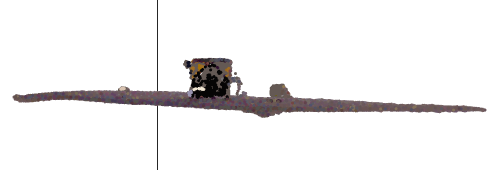
\includegraphics[height=1in]{plane_background_PCA}
        \caption{Background points lie almost within plane}
        \label{fig:plane_background_PCA}
    \end{subfigure}%
    ~ 
    \centering
    \begin{subfigure}[t]{0.45\textwidth}
        \centering
        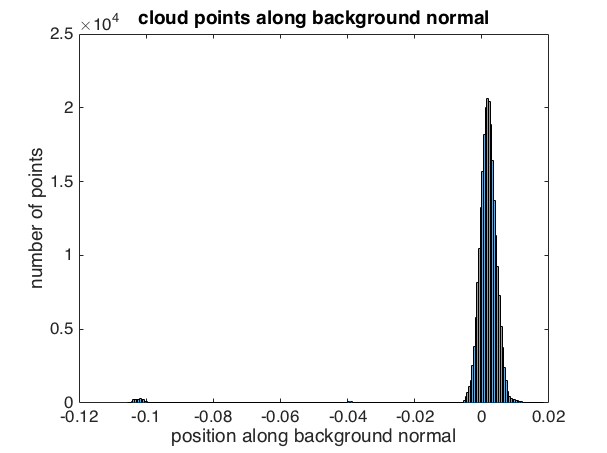
\includegraphics[height=2in]{projectedPositionsDist}
        \caption{Cloud points projected along background normal}
        \label{fig:projectedPositionsDist}
    \end{subfigure}
    \caption{}
\end{figure}

It relies on the observation that overwhelming majority of pixels belongs to the background. The background surface essentially can be approximated by plane as frames are recorded on smooth floor. It can be seen on Figure~\ref{fig:plane_background_PCA} where it is shown for the first frame. However, note that near the border cloud points of the background go slightly below the main plain. This happens presumably due to the imperfection of Kinect 3d sensor.  To extract plane we need to estimate normal of this plane and plane distance from origin of coordinate frame. 

First, we compute the normal to the background surface by applying PCA to centred cloud points. As we have 3D data we will receive 3 principal components. 1st and 2nd will be lying within surface of the background (because on the background surface the variety of coordinates is the greatest) and 3rd component will be orthogonal to them and, therefore it will be normal to the background surface. After that we project centred cloud points on background normal and get distribution where most of the points are concentrated on one level (background points near the surface of background plane). This distribution is shown on Figure~\ref{fig:projectedPositionsDist}. As we can see most of the points are located near one place along background normal axis (high peak near 0) and only relatively small amount of cloud points are located above the plane (small peak near -0.1). This confirms our hypothesis that background forms a plane. By taking 50th percentile of such distribution (basically it will give us location of the biggest peak because it dominates the data) we are able to find distance from origin of global coordinate frame.

Finally, we determine the correct direction of normal vector (where the spheres and cube cloud point lie) and remove all points which are located not high enough from surface plane. By doing that we are removing background cloud points near the border which go slightly below the main background plain. The results on this stage contain almost no points which belong to background. This is demonstrated on Figure~\ref{fig:substractedBackground1} for the first frame. The only exception occurs on 8th frame where we have  a few border outliers which lie above the main background plane. It can be seen on Figure~\ref{fig:frame_8_problem} where outliers are marked by red circle. But this is handled on the next stage.

\begin{figure}[htbp!]
    \centering
    \begin{subfigure}[t]{0.45\textwidth}
        \centering
        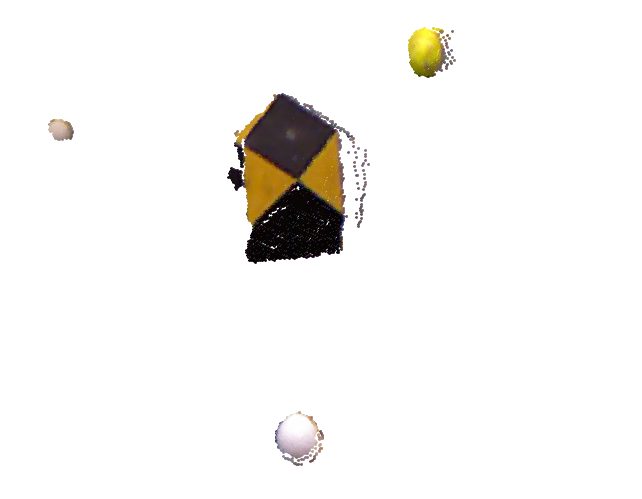
\includegraphics[height=2in]{substractedBackground1}
        \caption{Subtracted background for frame 1}
        \label{fig:substractedBackground1}
    \end{subfigure}%
    ~ 
    \centering
    \begin{subfigure}[t]{0.45\textwidth}
        \centering
        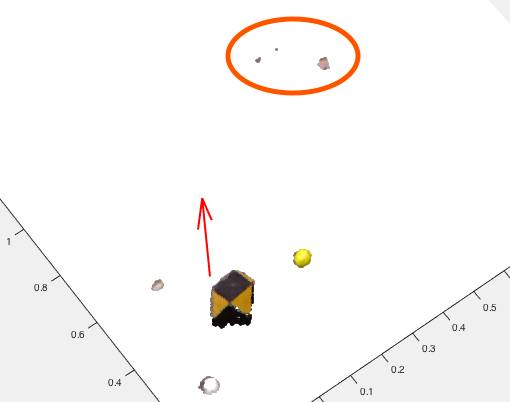
\includegraphics[height=2in]{frame_8_problem}
        \caption{Small number of border outliers on frame 8 marked by red circle}
        \label{fig:frame_8_problem}
    \end{subfigure}
    \caption{}
\end{figure}



\subsection{Clustering}

\begin{figure}[htbp!]
    \centering
    \begin{subfigure}[t]{0.45\textwidth}
        \centering
        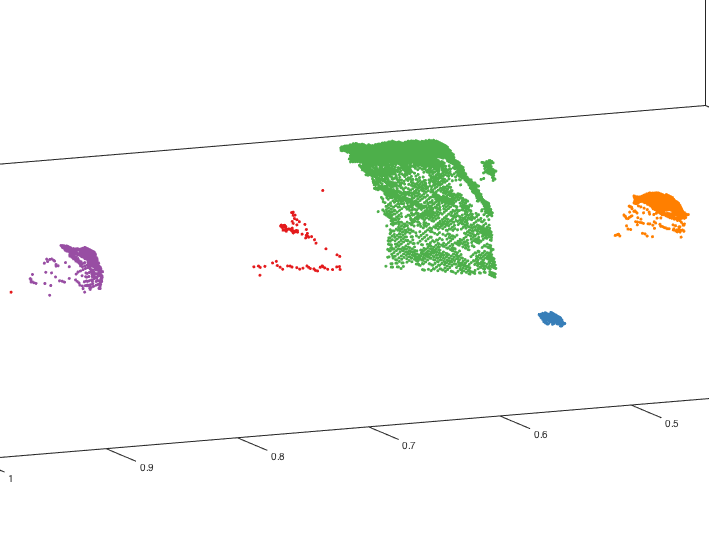
\includegraphics[height=2in]{clustering_outliers}
        \caption{Clustering with some noise marked as red}
        \label{fig:clustering_outliers}
    \end{subfigure}%
    ~ 
    \centering
    \begin{subfigure}[t]{0.45\textwidth}
        \centering
        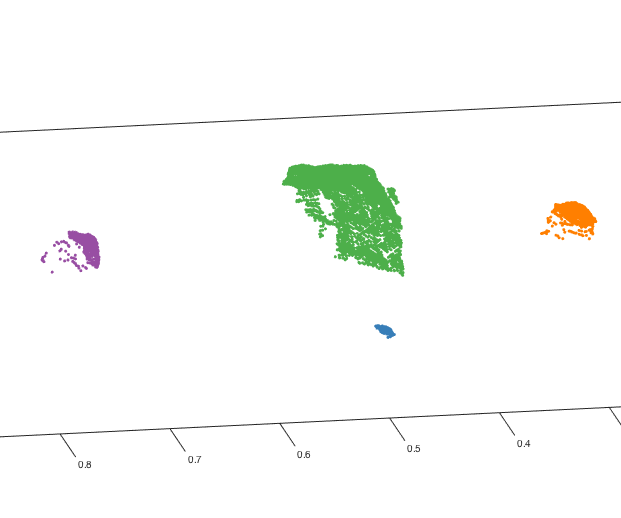
\includegraphics[height=2in]{clustering_without_outliers}
        \caption{After removing noise}
        \label{fig:clustering_without_outliers}
    \end{subfigure}
    \caption{}
\end{figure}


Here we determine the main clusters which potentially can be one of 4 objects we are interested in: 3 spheres or 1 cube. For that we are using Density-based spatial clustering of applications with noise (DBSCAN). The main advantage of this clustering algorithm to let's say kmeans is that it doesn't use explicit number of clusters and clusters are formed by connectivity to the nearest neighbours. Due to that it is possible to extract patches that forms very long shapes which allows to remove most of the noise (by offsetting minimal number points required to form cluster) located near the cube. This is demonstrated on Figures \ref{fig:clustering_outliers} and \ref{fig:clustering_without_outliers}. 

The parameters used for scanning:
\begin{itemize}
  \item number of objects in a neighbourhood of an object: \textbf{80}. Or in other words minimal size of the cluster. It was estimated empirically by printing number of points in located clusters which were matched to object of interests (on this stage by plotting the data). 
  \item neighbourhood radius: \textbf{0.015}. It was also estimated empirically by plotting clustering results (similarly to what can be seen on Figures \ref{fig:clustering_outliers} and \ref{fig:clustering_without_outliers}
\end{itemize}

Finally, the biggest cluster is located which must belong to cube. For example, the number of cloud points in the extracted clusters for the first frame:

 
\begin{center}
    \begin{tabular}{ |c|c|} 
        \hline
         cluster1 & 137 \\
         \hline
         cluster2 & 5050 \\
         \hline
         cluster3 & 442 \\
         \hline
         cluster4 & 796 \\
         \hline
        \end{tabular}
\end{center}

As we can see we have a cluster which has sufficiently more points as others. The same sitiuation holds for the rest of the frames.

Next, the remaining clusters are checked by proximity to the cube cluster. If they are too far way then they are recognised as border outliers and removed. If outliers were detected then after their removal additional clustering is used to get final results. This allows to remove border outliers from Figure~\ref{fig:frame_8_problem}. The implementation of DBscan is taken from \cite{dbscan}.

\section{Sphere extraction}

\begin{figure}[htbp!]
    \centering
    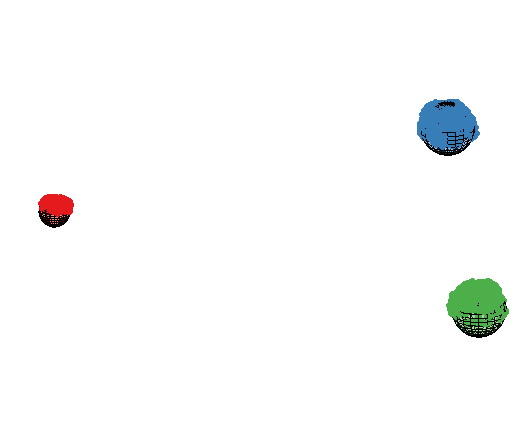
\includegraphics[height=3.3in]{spheres_allocated}
    \caption{Spheres fitted to ball patches for first frame}
    \label{fig:spheres_allocated}
\end{figure}

For all 16 frames once we located the biggest cluster (and we confirmed visually that indeed it corresponds to cube object) then we had only 3 other cluster which corresponded to the patches of ball cloud points. As extensions just in case we implemented searching of sphere clusters based on the idea that ball clusters will form triangle with the biggest area given that border outliers are successfully removed.

After that the spheres were fitted to the ball patches. This is shown on Figure \ref{fig:spheres_allocated}. Approximation of sphere centres proved to be reliable in the further stage when the final merging of cube data was done.

\section{Registration}
\subsection{Matching spheres to baseline frame}

\begin{figure}[htbp!]
    \centering
    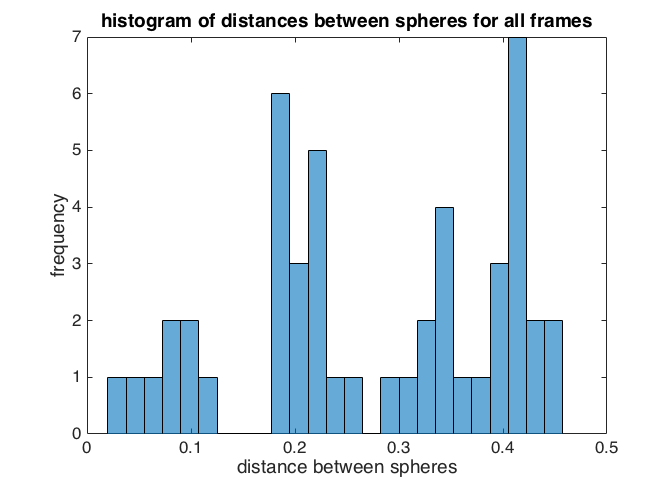
\includegraphics[height=3.3in]{histSphereDists}
    \caption{Distribution of distances between sphere for all frames}
    \label{fig:histSphereDists}
\end{figure}

We had several ideas on that. First we thought about using the length of triangle sides which is formed by the balls. Indeed, as it can be seen on Figure \ref{fig:histSphereDists} we can distinguish three different groups which corresponds to 3 different sides of triangle. Given that one of the balls is considerably smaller than others, potentially this method could be used. However, acknowledging the fact the last 2 groups can be very similar we decided to utilise colour information in order to distinguish between different balls. 
For that we computer colour histograms and calculated bhattacharyya distance between histograms for different frames in order to find right matches between balls. This can be done easily because in contrast to the first assignment colour histograms of each ball are very unique (there is no ambiguity between them). This is demonstrated on
Figures \ref{fig:color_hist_frame_1} and \ref{fig:color_hist_frame_1_orig}. Here colours of the lines mean only correspondence to the particular ball on Figure \ref{fig:color_hist_frame_1_orig} because all colour channels (red, green, blue) are concatenated to form single vector and normalised.

\begin{figure}[htbp!]
    \centering
    \begin{subfigure}[t]{0.85\textwidth}
        \centering
        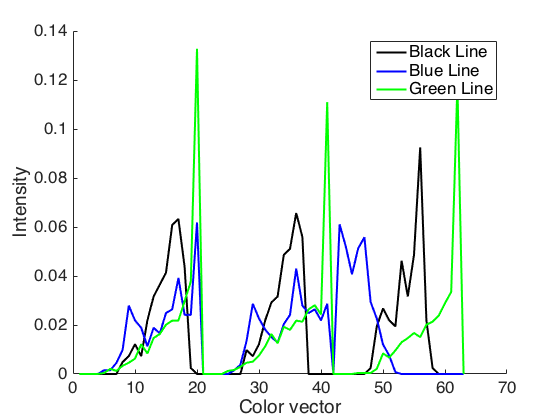
\includegraphics[height=4in]{color_hist_frame_1}
        \caption{Colour histograms (all channels are concatenated to form single vector and normalised)}
        \label{fig:color_hist_frame_1}
    \end{subfigure}%
    \\
    \centering
    \begin{subfigure}[t]{0.85\textwidth}
        \centering
        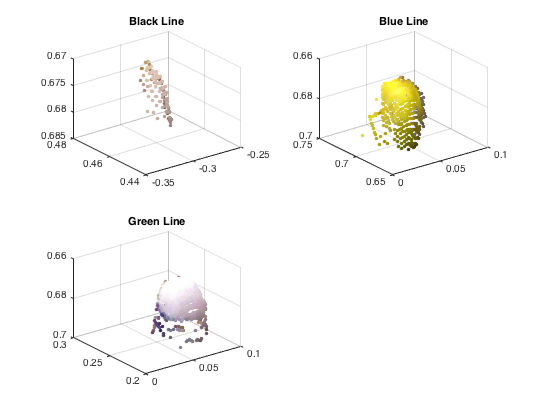
\includegraphics[height=4in]{color_hist_frame_1_orig}
        \caption{Corresponding balls from the first frame}
        \label{fig:color_hist_frame_1_orig}
    \end{subfigure}
    
    \caption{}
\end{figure}

Using colour histograms matching worked properly for all frames which was confirmed by next stage

\subsection{Merge Cube Points}

\begin{figure}[htbp!]
    \centering
    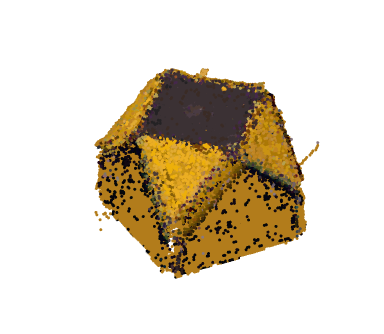
\includegraphics[height=3.3in]{mergedCube}
    \caption{merged cube cloud points}
    \label{fig:mergedCube}
\end{figure}

Using matches between different balls for different frames obtained from colour histograms the transformation to baseline frame was computing for all frames. Transformations were found with PCA to minimise mean square error between triangles positions and rotations formed by balls. The resulting merged cube is shown on Figure \ref{fig:mergedCube}. Note, that due to the clustering stage the resulting merged Cube has relatively small amount of noise.




\printbibliography[
    heading=bibintoc,
    title={References}
    ] %Prints the entire bibliography
    



\end{document}